% Copyright 2019 Clara Eleonore Pavillet

% Author: Clara Eleonore Pavillet (original author), Leonard Quentin Marcq (modified for tsinghua), 赵宗义 (参与了修改), Li(modified for PKU)
% Description: This is an unofficial Peking University Beamer Template I made from scratch. Feel free to use it, modify it, share it.
% Repo Address: https://github.com/synthpop123/PKU-Beamer-Template
% Version: 1.1.1


\documentclass{beamer}
\usepackage{ctex}
\usepackage{fontspec}
\usepackage{listings}
% Load Packages
\usepackage[utf8]{inputenc}
\usepackage{xcolor}
\usepackage{tikz}
\usetikzlibrary{positioning,calc}
\usepackage{graphicx}
\usepackage{hyperref}
\usepackage{amsmath}
\usepackage{listings}
%\usepackage{fontawesome}

% Define Commands
\newcommand*{\ClipSep}{0.06cm} %To adjust footer logo
\newcommand{\E}{\mathrm{e}\,} %\def\I{e} % used to defined e for exp(x), see later what it should be
\newcommand{\ud}{\mathrm{d}}
\lstset{numbers=left, numberstyle=\tiny, stepnumber=1,firstnumber=1,breaklines=true,
    numbersep=5pt,language=Python,
    stringstyle=\ttfamily,
    basicstyle=\footnotesize, 
    showstringspaces=false
}

\usetheme{pku}

%%%<<<---
\newcommand{\system}{ICS}
\newcommand{\variable}{\mathrm}
\newcommand{\field}{\mathsf}
%%%--->>>

\title{\textbf{ICS Midterm Review}}
\titlegraphic{
\includegraphics[width=2cm]{Theme/Logos/pku_emblem.png}}
\author{Yuxuan Kuang}
\institute{School of EECS, PKU}
\date{2022-10-26}

\begin{document}

{\setbeamertemplate{footline}{} 
\frame{\titlepage}}

\begin{frame}{2 Representing and Manipulating Information}
\textbf{Basic}
\begin{enumerate}
	\item Bit-level operations
	\item Integers
	\item Floating-point numbers
\end{enumerate}
\textbf{Enhanced}
\begin{enumerate}
	\item Big Endian and Little Endian, \textbf{string} % not confuse with stack attack!
	\item Casting: change the way of interpreting, \textbf{implicit}
	\item Overflow and roundings
	\item Special floating point numbers: \textbf{norm, denorm, inf, nan}
\end{enumerate}
\end{frame}

\begin{frame}{2 Representing and Manipulating Information}
	\begin{figure}
		\centering
		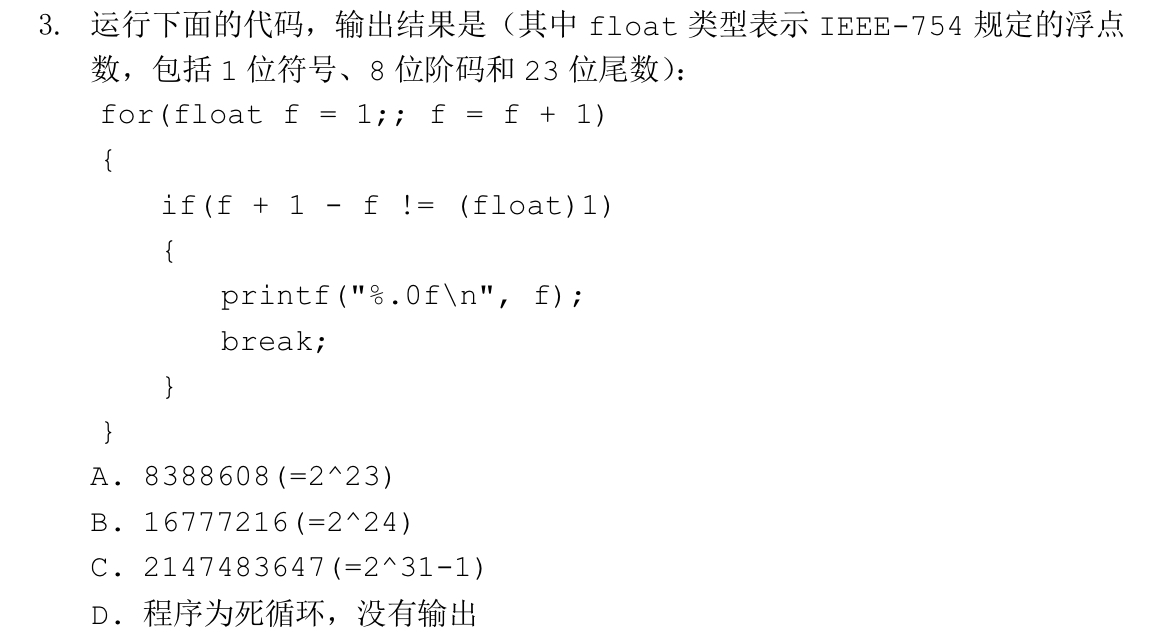
\includegraphics[width=1.0\textwidth]{figures/2-1.jpeg}
	\end{figure}
\end{frame}


\begin{frame}{3 Machine-Level Representation of C Programs}
\textbf{Basic}
\begin{enumerate}
	\item Program Encodings, registers
	\item Control
	\item Procedures
	\item Data
\end{enumerate}
\textbf{Enhanced}
\begin{enumerate}
	\item Alignment
	\item Arrays and Pointers, \textbf{complex and nested}
	\item Condition Codes: instructions*, combinations
	\item Misc: \textbf{sizeof*, jump* \& switch, RISC \& CISC, gdb}
\end{enumerate}
\end{frame}

\begin{frame}{3 Machine-Level Representation of C Programs}
	\begin{figure}
		\centering
		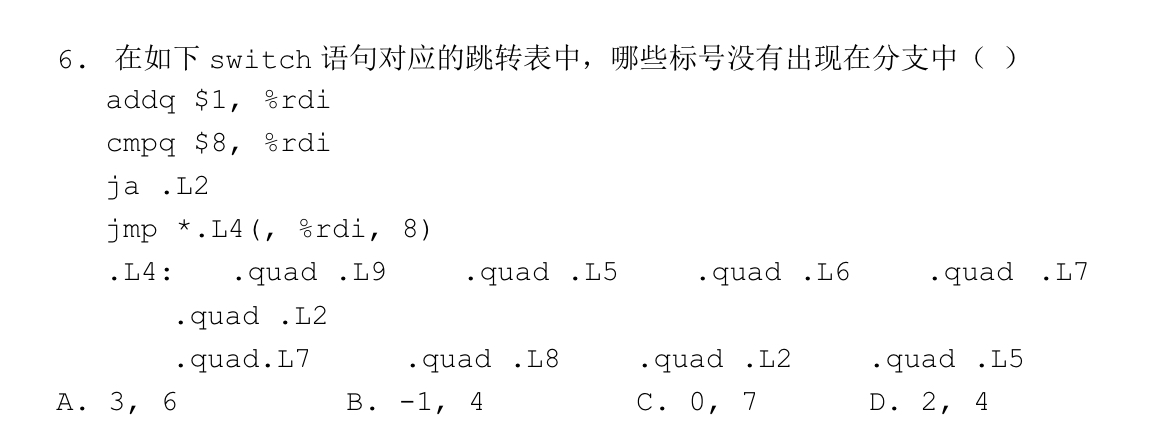
\includegraphics[width=1.0\textwidth]{figures/3-1.jpeg}
	\end{figure}
\end{frame}

\begin{frame}{3 Machine-Level Representation of C Programs}
	\begin{figure}
		\centering
		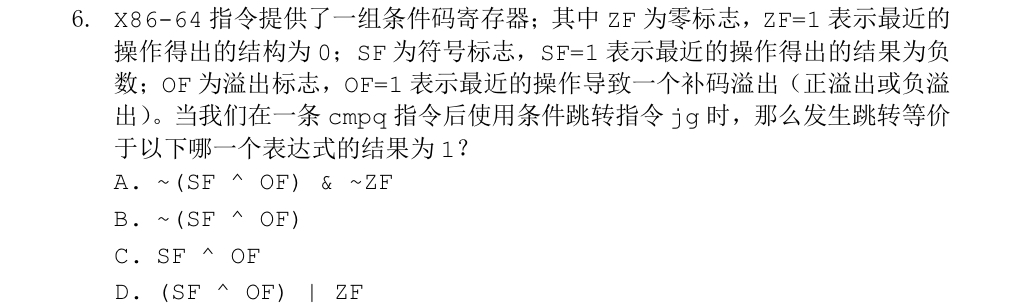
\includegraphics[width=1.0\textwidth]{figures/3-2.jpeg}
	\end{figure}
\end{frame}

\begin{frame}{4 Processor Architecture}
\textbf{Basic}
\begin{enumerate}
	\item Instruction Set Architecture
	\item Sequential Logic
	\item Pipeline
\end{enumerate}
\textbf{Enhanced: new instructions}
\begin{enumerate}
	\item Stages
	\item Pipeline correction, HCL
	\item Hazards
\end{enumerate}
\end{frame}

\begin{frame}{4 Processor Architecture}
	\begin{figure}
		\centering
		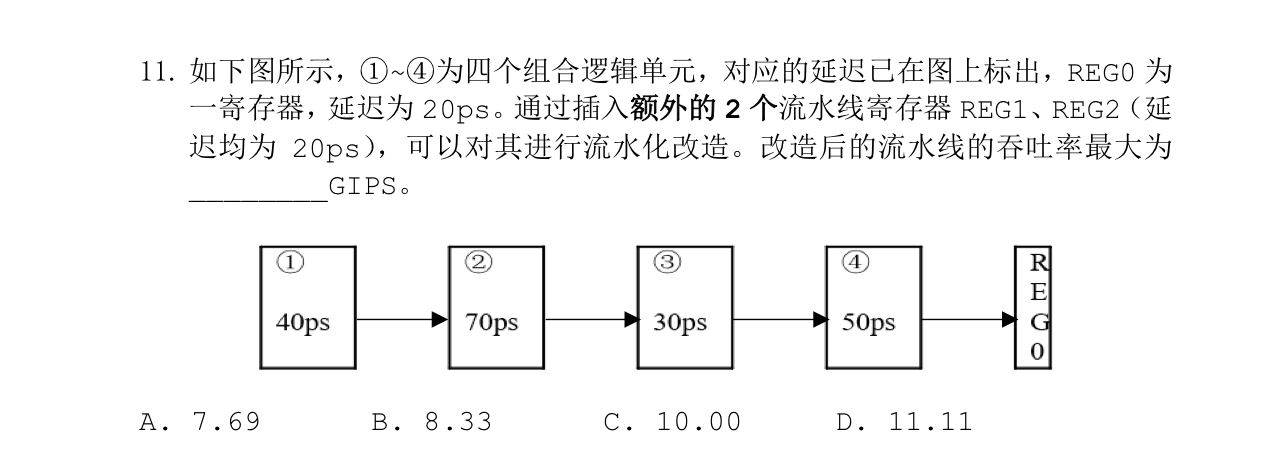
\includegraphics[width=1.0\textwidth]{figures/4-0.jpeg}
	\end{figure}
\end{frame}

\begin{frame}{4 Processor Architecture}
	New instruction: cretXX |9|fun|
	\begin{figure}
		\centering
		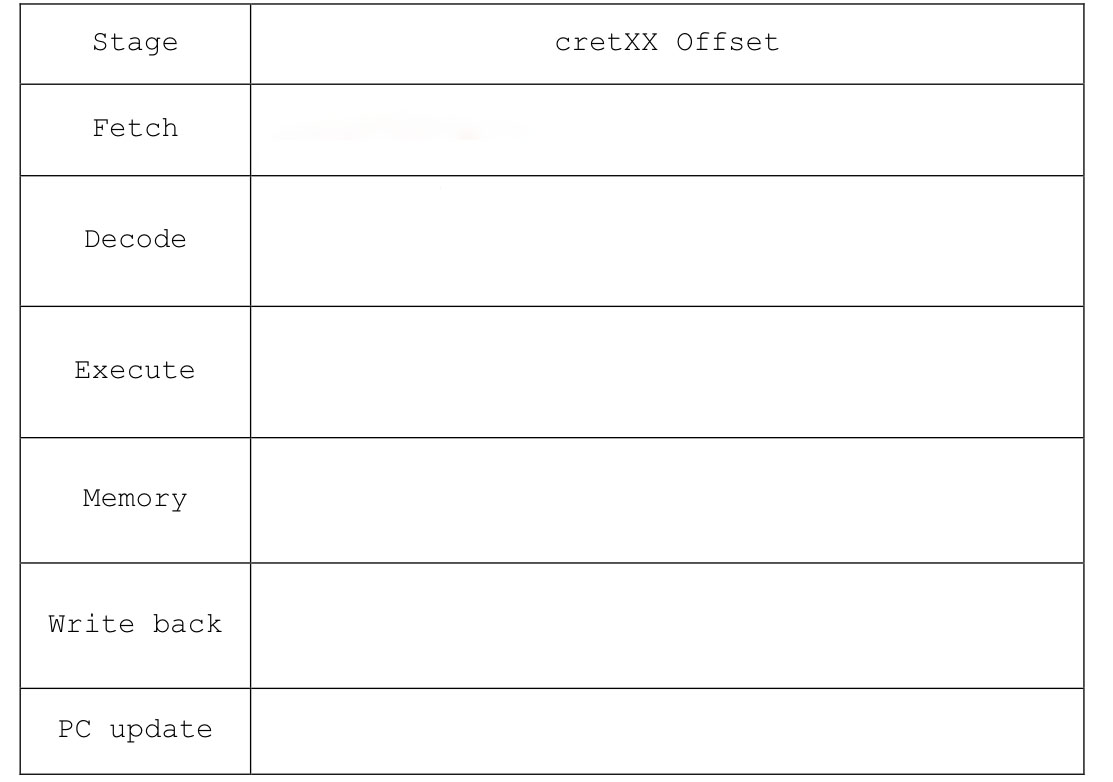
\includegraphics[width=0.8\textwidth]{figures/4-1-1.jpeg}
	\end{figure}
\end{frame}

\begin{frame}{4 Processor Architecture}
	New instruction: cretXX |9|fun|
	\begin{figure}
		\centering
		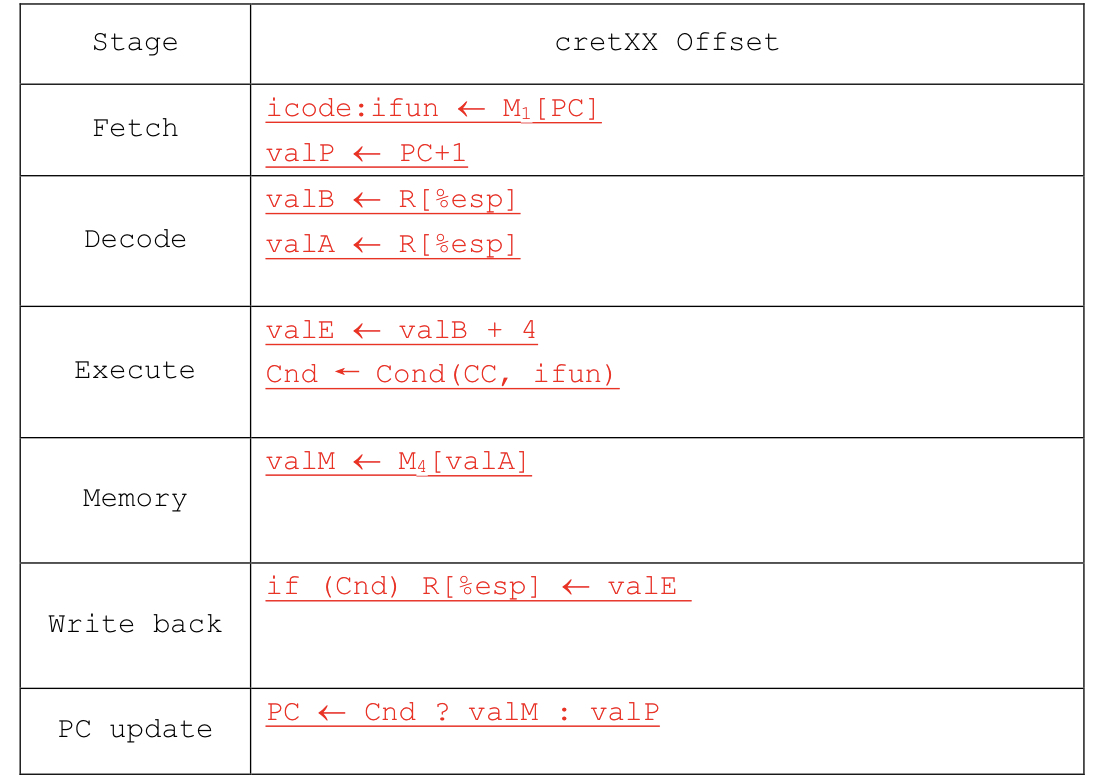
\includegraphics[width=0.8\textwidth]{figures/4-1-2.jpeg}
	\end{figure}
\end{frame}

\begin{frame}{5 Optimizing Program Performance}
\textbf{Basic}
\begin{enumerate}
	\item Performance Metrics and Analysis
	\item Loop Unrolling \& Parallelism
\end{enumerate}
\textbf{Enhanced}
\begin{enumerate}
	\item Modern Processors
	\item Memory Performance
\end{enumerate}
\end{frame}

\begin{frame}{5 Optimizing Program Performance}
	\begin{figure}
		\centering
		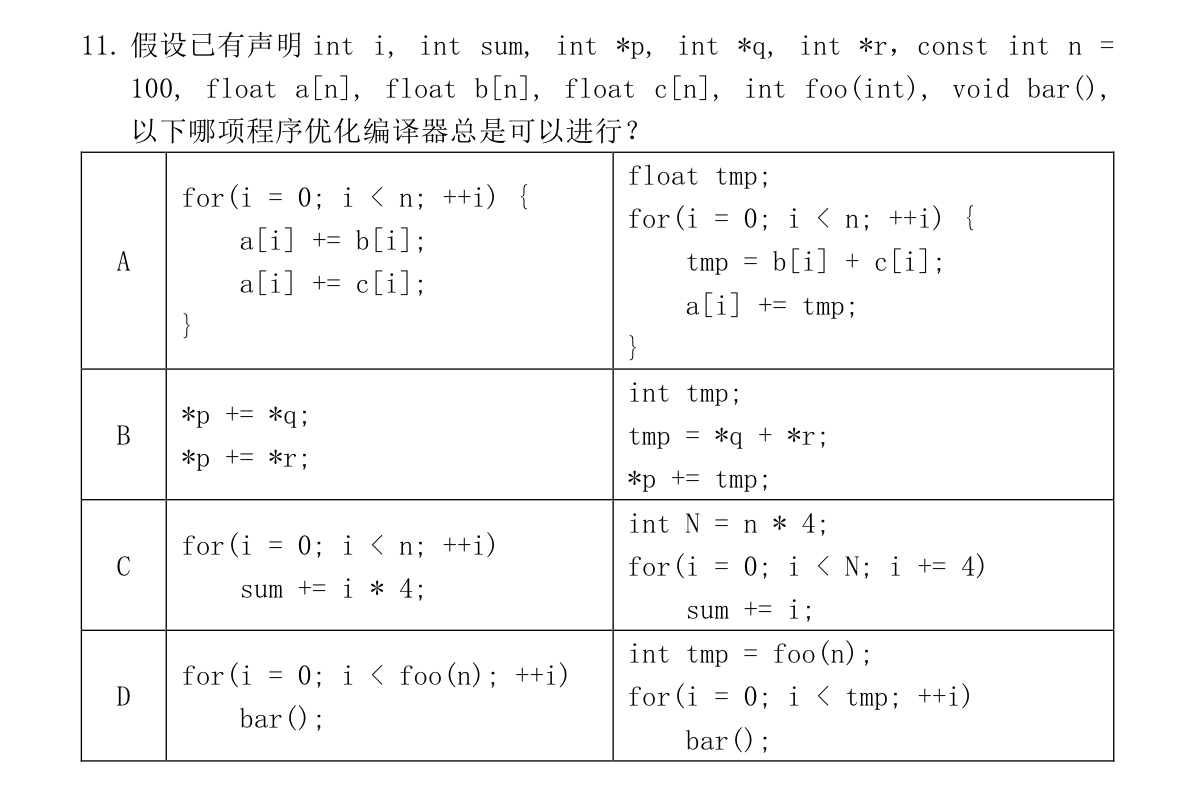
\includegraphics[width=0.9\textwidth]{figures/5-0.jpeg}
	\end{figure}
\end{frame}


\begin{frame}{6 The Memory Hierarchy}
\textbf{Basic}
\begin{enumerate}
	\item Memory Hierarchy
	\item Caches
\end{enumerate}
\textbf{Enhanced}
\begin{enumerate}
	\item Cache Organization: simutations and optimizations
	\item Locality
	\item Substitution Policies
\end{enumerate}
\end{frame}

\begin{frame}{6 The Memory Hierarchy}
	\begin{figure}
		\centering
		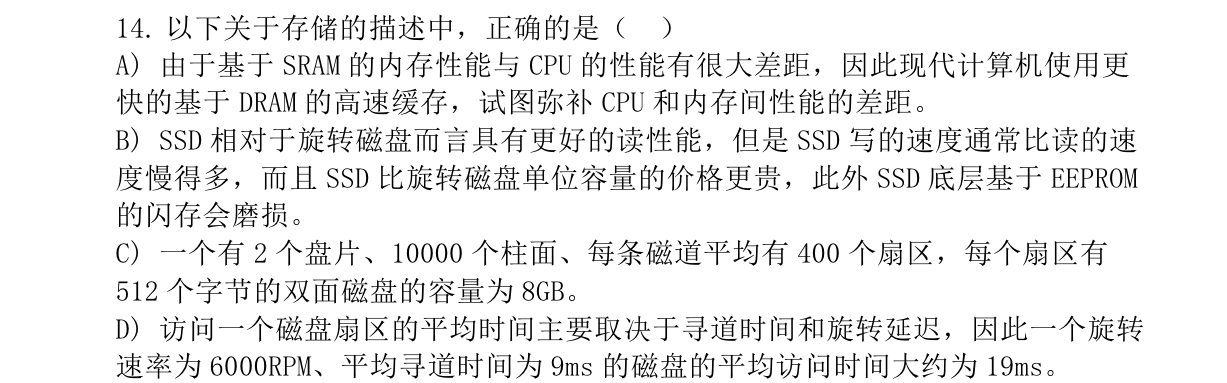
\includegraphics[width=1.0\textwidth]{figures/6-0.jpeg}
	\end{figure}
\end{frame}

\begin{frame}{6 The Memory Hierarchy}
	\begin{figure}
		\centering
		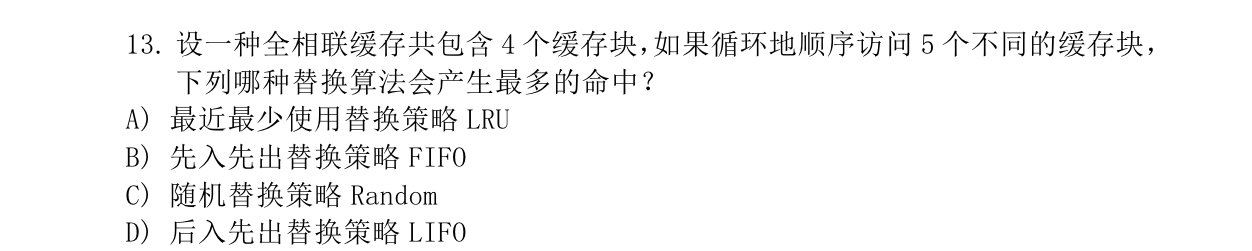
\includegraphics[width=1.0\textwidth]{figures/6-1.jpeg}
	\end{figure}
\end{frame}
  
\begin{frame}{}
\begin{center}
    \textbf{Thank you for your attention!}
\end{center}
\end{frame}


\end{document}

